\documentclass[aspectratio=43,english]{beamer} %If you want to create Polish presentation, replace 'english' with 'polish' and uncomment 3-th line, i.e., '\usepackage{polski}'
\usepackage[utf8]{inputenc}
\usepackage{polski} %Uncomment for Polish language
\usepackage{babel}
\usepackage{listings} %We want to put listings

\mode<beamer>{ 	%in 'beamer' mode
	\hypersetup{pdfpagemode=FullScreen}		%Enable Full screen mode
	\usetheme{JuanLesPins} 		%Show part title in right footer
	%\usetheme[dark]{AGH}                 		%Use dark background
	%\usetheme[dark,parttitle=leftfooter]{AGH}  	%Use dark background and show part title in left footer
}
\mode<handout>{	%in 'handout' mode
	\hypersetup{pdfpagemode=None}		
	\usepackage{pgfpages}
  	\pgfpagesuselayout{4 on 1}[a4paper,border shrink=5mm,landscape]	%show 4 slides on 1 page
  	\usetheme{boxes}
  	\addheadbox{structure}{\quad\insertpart\hfill\insertsection\hfill\insertsubsection\qquad} 	%content of header
 	\addfootbox{structure}{\quad\insertauthor\hfill\insertframenumber\hfill\insertsubtitle\qquad} 	%content of footer
}

\AtBeginPart{ %At begin part: display its name
	\frame{\partpage}
} 


%%%%%%%%%%% Configuration of the listings package %%%%%%%%%%%%%%%%%%%%%%%%%%
% Source: https://en.wikibooks.org/wiki/LaTeX/Source_Code_Listings#Using_the_listings_package
%%%%%%%%%%%%%%%%%%%%%%%%%%%%%%%%%%%%%%%%%%%%%%%%%%%%%%%%%%%%%%%%%%%%%%%%%%%%
\lstset{ %
  backgroundcolor=\color{white},   % choose the background color
  basicstyle=\footnotesize,        % the size of the fonts that are used for the code
  breakatwhitespace=false,         % sets if automatic breaks should only happen at whitespace
  breaklines=true,                 % sets automatic line breaking
  captionpos=b,                    % sets the caption-position to bottom
  commentstyle=\color{green},      % comment style
  deletekeywords={...},            % if you want to delete keywords from the given language
  escapeinside={\%*}{*)},          % if you want to add LaTeX within your code
  extendedchars=true,              % lets you use non-ASCII characters; for 8-bits encodings only, does not work with UTF-8
  frame=single,	                   % adds a frame around the code
  keepspaces=true,                 % keeps spaces in text, useful for keeping indentation of code (possibly needs columns=flexible)
  keywordstyle=\color{blue},       % keyword style
  morekeywords={*,...},            % if you want to add more keywords to the set
  numbers=left,                    % where to put the line-numbers; possible values are (none, left, right)
  numbersep=5pt,                   % how far the line-numbers are from the code
  numberstyle=\tiny\color{gray},   % the style that is used for the line-numbers
  rulecolor=\color{black},         % if not set, the frame-color may be changed on line-breaks within not-black text (e.g. comments (green here))
  showspaces=false,                % show spaces everywhere adding particular underscores; it overrides 'showstringspaces'
  showstringspaces=false,          % underline spaces within strings only
  showtabs=false,                  % show tabs within strings adding particular underscores
  stepnumber=2,                    % the step between two line-numbers. If it's 1, each line will be numbered
  stringstyle=\color{cyan},        % string literal style
  tabsize=2,	                   % sets default tabsize to 2 spaces
  title=\lstname,                  % show the filename of files included with \lstinputlisting; also try caption instead of title
                                   % needed if you want to use UTF-8 Polish chars
  literate={?}{{\k{a}}}1
           {?}{{\k{A}}}1
           {?}{{\k{e}}}1
           {?}{{\k{E}}}1
           {�}{{\'o}}1
           {�}{{\'O}}1
           {?}{{\'s}}1
           {?}{{\'S}}1
           {?}{{\l{}}}1
           {?}{{\L{}}}1
           {?}{{\.z}}1
           {?}{{\.Z}}1
           {?}{{\'z}}1
           {?}{{\'Z}}1
           {?}{{\'c}}1
           {?}{{\'C}}1
           {?}{{\'n}}1
           {?}{{\'N}}1
}
%%%%%%%%%%%%%%%%%


\title{Metody Obliczeniowe w Nauce i Technice}
\author{Marian Bubak, PhD}
\date{}
\institute[AGH]{
	Institute of Computer Science\\ul. Kawiory 21\\30-055 Krakow\\
	Poland\\
	\url{http://www.icsr.agh.edu.pl/~mownit/}
}



%%%%%%%%%%%%%%%%
\usepackage{amsmath}
\usepackage{setspace}
\usepackage{scrextend}
%%%%%%%%%%%%%%%%

\subtitle{2. Arytmetyka komputerowa}
\setcontributors{Maciej Trzebiński\\Mikołaj Biel}

\begin{document}
  	\maketitle
	%%%%%%%%%%%%%%%%
	\begin{frame}{Outline}
		\tableofcontents
	\end{frame}
	%%%%%%%%%%%%%%%%
	\section{Numeryczna reprezentacja liczb całkowitych}
%%%%%%%%%%%%%%%%
\begin{frame}{Reprezentacja stałopozycyjna (integer)}
	\textcolor{blue}{Informacje ogólne:}
	\begin{itemize}
		\item np. kod U2: na d+1 bitach reprezentowane dokładnie liczby
			\begin{center}
				\[
   					 L \in [-2^d, 2^d-1]
    			\]
			\end{center}
		\item gdy argumenty i wynik reprezentowane stałopozycyjnie, to działania na nich: $+$, $-$, $\cdot$, $/ (div)$, $/ (mod)$ są wykonywane dokładnie
		\item kompromis pomiędzy zakresem, a precyzją
		
	\end{itemize}
     
\end{frame}
%%%%%%%%%%%%%%%%
\begin{frame}    
    
    \textbf{Zastosowania:}
    \begin{itemize}
    	\item sprawy walutowe, operacje monetarne
    	\item procesory graficzne np. Sony Nintendo
    	\item rozmiary czcionek w calach np. w TeX
    	\item libfixmath - implementacja biblioteki stałoprzecinkowej w C
    \end{itemize}
    $\newline$
    \textbf{Zalety i wady:}
    \begin{itemize}
    	\item (+) szybkość i prostota
    	\item (-) mała skalowalność
    \end{itemize}
\end{frame}
%%%%%%%%%%%%%%%%
	%%%%%%%%%%%%%%%%
	\section{Numeryczna reprezentacja liczb rzeczywistych}
%%%%%%%%%%%%%%%%
\begin{frame}{Reprezentacja zmiennoprzecinkowa (float)}
    Należy pamiętać o ułomności reprezentacji zbioru liczb rzeczywistych $\mathbb{R}$ w rzeczywistym świecie skończonych komputerów.
    \begin{block}{}
    $F$ - zbiór liczb zmiennoprzecinkowych (floating-point):\newline
    \begin{columns}
        \column{0.45\linewidth}
            $\beta$ - podstawa,\newline
            $t$ - dokładność,\newline
            $L, U$ - zakres wykładnika\newline
        \column{0.45\linewidth}
            $d_i$ - liczby całkowite,
            $0 \le d_i \le \beta - 1, i=1,...,t$
            $L \le e \le U$
    \end{columns}
    $x \in F$ ma wartość:
    \[
    x = \pm \underbrace{\left(\frac{d_1}{\beta} + \frac{d_2}{\beta^2} + ... + \frac{d_t}{\beta^t}\right)}_\text{mantysa} \cdot \beta^{\overbrace{e}^\text{cecha}}
    = \pm \sum_{i=1}^{t} \frac{d_i}{\beta^i} \cdot \beta^e
    \]        
    System $F$ jest {\it unormowany}, gdy $\forall_{x \ne 0}\ d_i \ne 0$.
    \end{block}

\end{frame}
%%%%%%%%%%%%%%%%
\begin{frame}{Reprezentacja zmiennoprzecinkowa (float)}
    W komputerze jest przechowywana liczba całkowita $\pm\beta^t \cdot m$ (zgodnie z wybranym systemem kodowania).
	$\newline$$\newline$
    $\beta^{1-t}$ - oszacowanie względnej dokładności arytmetyki

    \hspace{0.5cm}
    \centering
    \begin{tabular}{| l | c | c | c | c | c |}
    \hline
    Komputer & $\beta$ & $t$ & $L$ & $U$ & $\beta^{1-t}$ \\ \hline
    CDC CYBER 72 		& 2  & 48 & -975 	& 1070 & $7.11 \cdot 10^{-15}$ \\ \hline
    Cray-1 				& 2  & 48 & -16384	& 8191 & $7.11 \cdot 10^{-15}$ \\ \hline
    IBM 360, 370 		& 16 & 6  & -64		& 63   & $9.54 \cdot 10^{-7}$ \\ \hline
    IBM 360, 370 (DP) 	& 16 & 14 & -64 	& 63   & $2.22 \cdot 10^{-16}$ \\ \hline
    IBM PC XT / AT 		& & & & & \\ \hline
    Delta (VAX) 		& & & & & \\ \hline
    \end{tabular}
\end{frame}
%%%%%%%%%%%%%%%%
\begin{frame}{Reprezentacja zmiennoprzecinkowa (float)}
    \begin{block}{Ważne}
    $F$ nie jest kontinuum - więcej - jest skończony o liczbie elementów wyrażonych wzorem:
    \[
    2 \cdot \left(\beta - 1 \right) \cdot \beta^{t-1} \cdot \left( U - L + 1 \right) + 1
    \]
    \begin{flushright}
    \end{flushright}
    \end{block}
    \textcolor{blue}{Wyjaśnienie:}
    \begin{itemize}
    	\item 2 $\rightarrow$ znak liczby $\pm$
    	\item  $(\beta - 1)$ $\rightarrow$ podstawa, na pierwszym bicie nie ma zera
    	\item $\beta^{t-1}$ $\rightarrow$ pozostałe t-1 bitów z przedziału ${0,\dots,\beta-1}$
    	\item $(U - L + 1)$ $\rightarrow$ zakres wykładnika
    	\item 1 $\rightarrow$ zero
    \end{itemize}
    
\end{frame}
%%%%%%%%%%%%%%%%
\begin{frame}{Reprezentacja zmiennoprzecinkowa (float)}
    Elementy $F$ nie są równomiernie rozłożone na osi:
    $\beta = 2, t = 3, L = -1, U = 2$ \hspace{5mm} (33 elementy):
    \begin{center}
    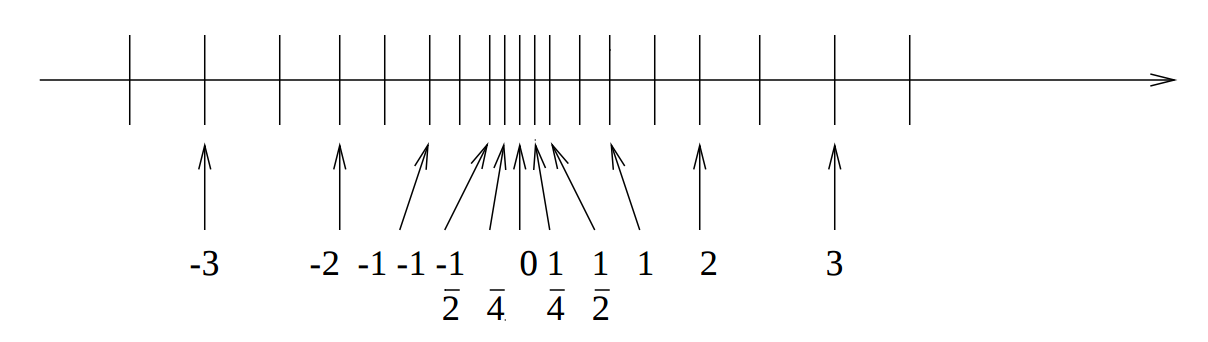
\includegraphics[width=0.8\linewidth]{img/2/2_1_axis}
    \end{center}

    Każdy element $F$ reprezentuje cały przedział liczb $\mathbb{R}$\newline 
    $x$ - l. rzeczywista $\in$ zakresu $F$,\newline
    $fl(x)$ - reprezentacja zmiennoprzecinkowa liczby $x$

    \[
    \left| \frac{fl(x) - x}{x} \right| \le \frac{1}{2} \beta^{1-t}
    \]

    \begin{flushright}
        {\it Zadanie:} sprawdzić
    \end{flushright}
\end{frame}
%%%%%%%%%%%%%%%%
\begin{frame}{Reprezentacja zmiennoprzecinkowa (float)}
    \begin{alertblock}{Uwaga}
        $0.1$ - często krok w algorytmach\newline
        Czy 10 kroków o długości $0.1$ to to samo co 1 krok = $1.0$?\newline\newline
        W systemie o podstawie $\beta = 2$ - {\bf nie!}
        \[
        0.1_{10} = 0.0(0011)_2 = 0.0(12)_4 = 0.0(6314)_8 = 0.199999..._{16}
        \]

        Reprezentacja $0.1$ urywa się po $t$ cyfrach. Dodanie 10 tak uzyskanych liczb nie da dokładnie $1.0$.
    \end{alertblock}
    
    \begin{alertblock}{Porównania w arytmetyce float}
    Zamiast przyrównywać wartości należy sprawdzać, czy otrzymany błąd pomiędzy wartością obliczoną, a oczekiwaną jest mniejszy od zadanego $\epsilon$.
    \end{alertblock}
\end{frame}
%%%%%%%%%%%%%%%%
\subsection{Dokładność reprezentacji zmiennoprzecinkowej}
\begin{frame}{Reprezentacja zmiennoprzecinkowa (float)}
    \[
    x = s \cdot 2^c \cdot m
    \]
    \begin{center}
    s $\leftarrow$ sign,\ c$\leftarrow$ cecha,\ m $\leftarrow$ mantysa
    \end{center}
    \[
    m = \sum_{i=1}^{\infty} e_i \cdot 2^{-i}
    \]\[
    e_i = \left\{ 
              \begin{array}{ll}
                  0 \\
                  1
              \end{array}
        \right.
    \]

    \begin{block}{Reprezentacja mantysy}
        $$
        m_t = \underbrace{\sum_{i=1}^{t}e_i \cdot 2^{-i}}_\text{t-bitowa mantysa} \ + \underbrace{e_{t+1} \cdot 2^{-t}}_\text{zaokrąglenie}
        $$
    \end{block}
\end{frame}
%%%%%%%%%%%%%%%%
\begin{frame}{Reprezentacja zmiennoprzecinkowa (float)}
    a)Błąd reprezentacji zmiennoprzecinkowej - zaokrąglenie w dół\newline
	$$
		fl(x)^{-} = \pm \sum_{i=1}^{t}{\frac{d_{i}}{\beta_{i}}}\ \cdot \  \beta^e
	$$
    \centering
    \begin{tabular}{|*{5}{p{.75cm}|}}
        \hline
        t & t+1 & t+2 & ... &  \\ \hline
          & 0   & 1   & ... & 1 \\ \hline
    \end{tabular}
    \[
    m = \underbrace{\sum_{i=1}^{t} e_i \cdot 2^{-i} + 0 \cdot 2^{-(t+1)}}_{m_t} +
        \underbrace{\sum_{i=t+2}^{\infty} 1 \cdot 2^{-i}}_{
            \frac{1}{2^{t+1}} = 2^{-(t+1)}
        }
    \] \[
    m - m_t = 2^{-(t+1)}
    \]
\end{frame}
%%%%%%%%%%%%%%%%
\begin{frame}{Reprezentacja zmiennoprzecinkowa (float)}
    b)Błąd reprezentacji zmiennoprzecinkowej - zaokrąglenie w górę\newline
	$$
		fl(x)^{+} = \pm \sum_{i=1}^{t}{\frac{d_{i}}{\beta_{i}}}\ \cdot \  \beta^e \ \pm \frac{d_{t+1}}{\beta_{t+1}}
	$$	
    \centering
    \begin{tabular}{|*{5}{p{.75cm}|}}
        \hline
        t & t+1 & t+2 & ... &  \\ \hline
          & 1   & 0   & ... & 0 \\ \hline
    \end{tabular}
    \[
    m = \sum_{i=1}^{t} e_i \cdot 2^{-i} + 2^{-(t+1)}
    \]\[
    m_t = \sum_{i=1}^{t} e_i \cdot 2^{-i} + 2^{-t}
    \] \[
    m_t - m = 2^{-(t+1)}  \ \ \left| \frac{m - m_t}{m} \right| \le \frac{2^{-(t+1)}}{1/2} = 2^{-t}
    \]
\end{frame}
%%%%%%%%%%%%%%%%
\begin{frame}
	\textbf{Standaryzacja:}
	\begin{itemize}
		\item Reprezentacja zmiennoprzecinkowa została ustandaryzowana w celu ujednolicenia obliczeń
		\item IEEE754 - 1985; IEEE754 - 2008 
		\item treść standardu IEEE754-2008:$\newline$ \url{www.dsc.ufcg.edu.br/~cnum/modulos/Modulo2/IEEE754_2008.pdf}
		\item wywiad z jednym z twórców standardu IEEE754-1985 (William Kahan):\ \url{www.goo.gl/AeNLrd}
	\end{itemize}
	\textbf{Istotne pojęcia:}$\newline$
	\textit{ukryta jedynka, normalizacja mantysy, liczby zdenormalizowane}
\end{frame}
%%%%%%%%%%%%%%%%

	%%%%%%%%%%%%%%%%
	\section{Operacje zmiennopozycyjne}
%%%%%%%%%%%%%%%%
\begin{frame}{Operacje zmiennopozycyjne}
    $x, y \in F$ \newline
    $x + y \in^? F$

    \begin{center}
    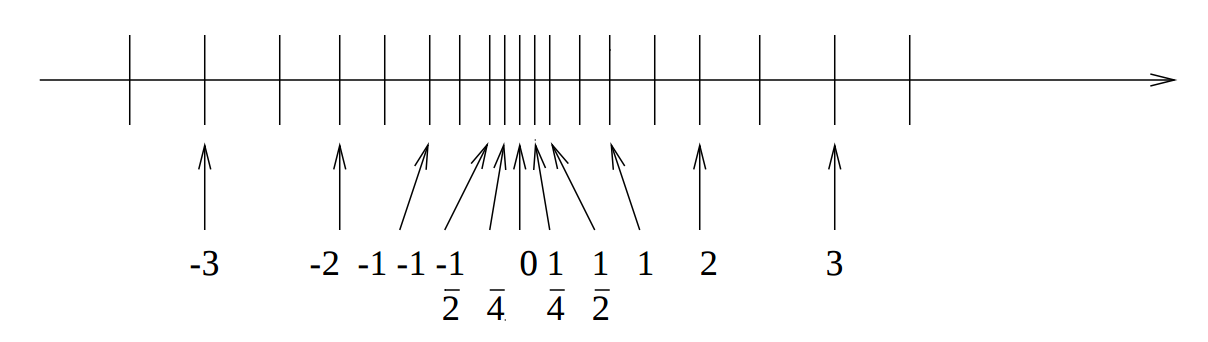
\includegraphics[width=0.8\linewidth]{img/2/2_1_axis}
    \end{center}
    System z powyższego rysunku: $\frac{5}{4} + \frac{3}{8} \notin F$ - ze względu na ,,gęstość'' elementów $F$.
\end{frame}
%%%%%%%%%%%%%%%%
\begin{frame}{Operacje zmiennopozycyjne}
    $\frac{7}{2} + \frac{7}{2} \notin F$ - {\it overflow}
    \vspace{.5cm}

    W większości komputerów: $x \oplus y = fl(x + y)$ dla $x + y$ z zakresu $F$

    $\oplus$ - dodawanie zmiennopozycyjne, \newline
    $fl$ - reprezentacja

    \[
    a + b = 2^{c_a} \cdot \left( m_a + m_b \cdot 2^{-(c_a-c_b)} \right) \Rightarrow
    \left\{ 
        \begin{array}{ll}
            |b| \le 1/2 \cdot 2^{-t} \cdot |a| \\
            fl(a + b) = a
        \end{array}
    \right.
    \]
\end{frame}
%%%%%%%%%%%%%%%%
\begin{frame}{Operacje zmiennopozycyjne}
    $x + y$ rzadko $\in F$, bo:
    \begin{itemize}
    \item $x \cdot y$ ma $2 \cdot t$ lub $2 \cdot t - 1$ cyfr znaczących,
    \item {\it overflow} - bardziej prawdopodobny
    \item {\it underflow} - bardziej prawdopodobny
    \item $\oplus, \odot$
        \begin{itemize}
        \item są {\it przemienne}
        \item nie są {\it łączne}, {\it rozdzielne}
        \end{itemize}
    \end{itemize}
\end{frame}
%%%%%%%%%%%%%%%%
\begin{frame}{Operacje zmiennopozycyjne}
    Ogólnie:
    \[
    fl(a \square b) = rd(a \square b) = (a \square b) \cdot (1 + \varepsilon)
    \] \[
    \varepsilon = \varepsilon(a, b, \square), \varepsilon \le \beta^{1-t}
    \] \[
    \square = +, -, \cdot, /
    \]

    \begin{block}{Definicja}
        {\bf Maszynowe $\varepsilon$} - najmniejsza liczba zmiennoprzecinkowa, dla której jeszcze: \[
        1 \oplus \varepsilon > 1
        \]
    \end{block}

    Zwykle wystarcza znajomość $\varepsilon' = 2^k \cdot \varepsilon, k \approx 1, 2, 3, ...$ $\rightarrow$ fragment progr. $\varepsilon$
\end{frame}
	%%%%%%%%%%%%%%%%
	\section{Zadanie, algorytm}
\begin{frame}{Zadanie, algorytm}
    \begin{block}{Definicja}
        \begin{columns}
            \column{.5\linewidth}
                \hfill dla danych
                \newline

                \hfill znaleźć wynik
            \column{.5\linewidth}
                $\vec{d} = \left( d_1, d_2, ..., d_n \right) \in R_d$\newline
                $\vec{w} = \left( w_1, w_2, ..., w_m \right) \in R_w$\newline
                $\vec{w} = \varphi(\vec{d})$
        \end{columns}
        $R_d$, $R_w$ - skończenie wymiarowe, unormowane przestrzenie kartezjańskie\newline
        $\varphi: D_0 \subset R_d \rightarrow R_w$ - odwzorowanie ciagłe
    \end{block}
    \begin{block}{Definicja}
        {\bf Algorytm A w klasie zadań $\{\varphi, D\}$} jest to sposób wyznaczenia wyniku $\vec{w} = \varphi(\vec{d})$ dla $d \in D \subset D_0$, z dokładną realizacją działań, tj. w zwykłej arytmetyce
    \end{block}
\end{frame}
%%%%%%%%%%%%%%%%
\begin{frame}{Realizacja algorytmu w arytmetyce fl - $fl(A(\vec{d}))$}
    zastąpienie:
    \begin{itemize}
        \item $d, x, ..$
        \item arytmetyki
    \end{itemize}
    przez:
    \begin{itemize}
        \item $rd(d), rd(x), ..$
        \item arytmetykę float
    \end{itemize}
\end{frame}
%%%%%%%%%%%%%%%%
\begin{frame}{Założenia o reprezentacji danych i wyników}
    \begin{block}{Założenia}
    \[
    || \vec{d} - rd(\vec{d}) ||
    \le 
    \varrho_d ||\vec{d} ||
    \] \[
    || \vec{w} - rd(\vec{w}) ||
    \le 
    \varrho_w ||\vec{w} ||
    \] \[
    \varrho_d, \varrho_w = \underbrace{k}_{\text{małe, } \approx 10} \cdot \beta^{1-t}
    \]
    \end{block}
    - reprezentowane z małymi błędami.
\end{frame}

	%%%%%%%%%%%%%%%%
	\section{Uwarunkowanie zadania ({\it condition of a problem})}
%%%%%%%%%%%%%%%%
\begin{frame}{Uwarunkowanie zadania}

	{\it Przyczyna:} zamiast 
    	$d_i \rightarrow rd(d_i) = d_i \cdot (1 + \varepsilon)$,
        $||\varepsilon|| \le \beta^{1-t}$
        
    \begin{block}{Definicja}
    	{\bf Uwarunkowanie zadania} - czułość na zaburzenie danych,
        
        {\bf Wskaźniki uwarunkowania zadania} - wielkości charakteryzujące wpływ zaburzeń danych zadania na zaburzenie jego rozwiązania.
    \end{block}
    
    \begin{block}{Definicja}
    Zadanie nazywamy źle uwarunkowanym, jeżeli niewielkie względne zmiany danych zadania powodują duże względne zmiany jego rozwiązania.
    \end{block}
\end{frame}
%%%%%%%%%%%%%%%%
\begin{frame}{Uwarunkowanie zadania}
	\begin{exampleblock}{Przykład}
    \begin{columns}
    	\column{.45\linewidth} 
        	\centering
            $\vec{x} \cdot \vec{y} = \sum_{i=1}^n x_i \cdot y_i \neq 0$
        \column{.45\linewidth} 
                $x_i \rightarrow x_i \cdot (1 + \alpha_i)$ \\
                $y_i \rightarrow y_i \cdot (1 + \beta_i)$
    \end{columns}
    \begin{gather*}
    	\underbrace{\left| \frac{
        	\sum_{i=1}^n x_i \cdot (1 + \alpha_i) \cdot y_i \cdot (1 + \beta_i) - \sum_{i=1}^n x_i y_i
        }{
        	\sum_{i=1}^n x_i \cdot y_i
        }\right|}_\text{błąd względny}
        \approx \\ \approx
        \left| \frac{
        	\sum_{i=1}^n \cdot x_i \cdot y_i \cdot \left( \alpha_i + \beta_i \right)
        }{
        	\sum_{i=1}^n x_i \cdot y_i
        }\right|
        \le
        \max \left| \alpha_i + \beta_i \right| \cdot \underbrace{\frac{
        	\sum_{i=1}^n \left| x_i \cdot y_i \right|
        }{
        	\left| \sum_{i=1}^n x_i \cdot y_i \right|
        }}_{cond(\vec{x} \cdot \vec{y})}
    \end{gather*}
    gdzie $cond(\vec{x} \cdot \vec{y})$ oznacza {\it wskaźnik uwarunkowania}, \\ 
    gdy wszystkie $x_i, y_i$ tego samego znaku $\Rightarrow cond(\vec{x} \cdot \vec{y}) = 1$
    \end{exampleblock}
\end{frame}
%%%%%%%%%%%%%%%%
\begin{frame}{Uwarunkowanie zadania}

	{\bf Poprawa:}
    \begin{itemize}
    	\item silniejsza arytmetyka,
        \item użycie zadania równoważnego
    \end{itemize}
\end{frame}
%%%%%%%%%%%%%%%%
	%%%%%%%%%%%%%%%%
	\section{O uwarunkowaniu zadania - inaczej}
%%%%%%%%%%%%%%%%
\begin{frame}{Jakościowo}
	Układ dwóch równań graficznie: \\
    niezależnie od jakości ołówka (algorytm) - lewa strona - dokładniej.
    
    \vspace{.5cm}
    \begin{columns}
    \column{.5\linewidth}
    	\centering   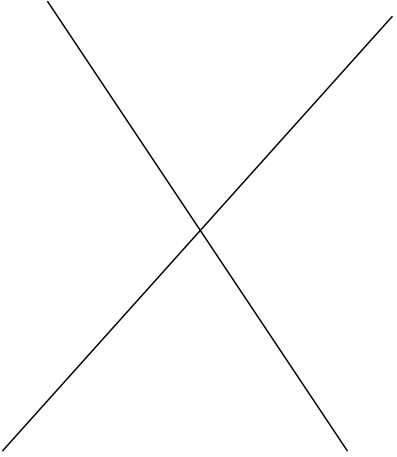
\includegraphics[width=.7\linewidth]{img/2/2_2_well_conditioned}
    \column{.5\linewidth}
    	\centering   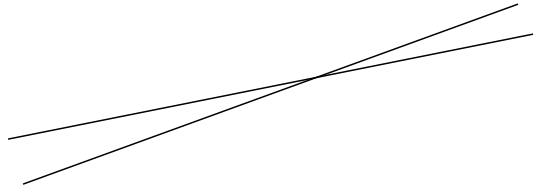
\includegraphics[width=.7\linewidth]{img/2/2_3_ill_conditioned}
    \end{columns}
    \vspace{.5cm}
    \begin{columns}
    \column{.5\linewidth}
    	\centering   well conditioned
    \column{.5\linewidth}
    	\centering   ill conditioned
    \end{columns}
\end{frame}
%%%%%%%%%%%%%%%%
\begin{frame}{Ilościowo}

	{\it Zadanie:} wyznaczenie $f(x)$,\ przy założeniu: $x^{*}$ - blisko $x$ \\
	$\newline$
    Współczynnik uwarunkowania:
    
    \vspace{.5cm}
    \centering
    \begin{tabular}{r c}
    	ogólnie: & \(
            K(x) = \lim_{x^{*} \to x} \frac{
                \left| \frac{
                    f(x) - f(x^{*})
                }{
                    f(x)
                } \right|
            }{
                \left| \frac{
                    x - x^{*}
                }{
                    x
                } \right|
            } = \left| \frac{
                x \cdot f'(x)
            }{
                f(x)
            } \right|
        \)\\
        
        $f(x) = \sqrt{x}$: & \(
        	K(x) = \left| \frac{
                x \cdot \frac{1}{2 \sqrt{x}}
            }{
                \sqrt{x}
            }\right| = \frac{1}{2}
        \) \\
        
        $f(x) = \frac{1}{1 - x}$: & \(
            K(x) = \frac{ \left|
                x \cdot \frac{1}{
                    (1-x)^2
                } \right| 
            }{ \left| 
                \frac{1}{1 - x}
            \right| } = \frac{x}{1 - x}
          	\) \\
            & \(
            x = (1 + 10^{-6}) \Rightarrow K \approx 10^6 \hspace{.5cm} (!)
            \)
    \end{tabular}
\end{frame}
%%%%%%%%%%%%%%%%
	%%%%%%%%%%%%%%%%
	\section{Uwarunkowanie zadania - przykład}
%%%%%%%%%%%%%%%%
\begin{frame}{Uwarunkowanie zadania - przykład}
	\begin{exampleblock}{Przykład 1}
    	\[
        	(x-2)^2 = 10^{-6} \Rightarrow x_\text{1, 2} = 2 \mp 10^{-3}
        \]
        {\bf ALE:} zmiana stałej o $10^{-6} \rightarrow$ zmiana $x_\text{1, 2}$ o $10^{-3}$!
    \end{exampleblock}
\end{frame}
%%%%%%%%%%%%%%%%
\begin{frame}{Uwarunkowanie zadania - przykład}
	\begin{exampleblock}{Przykład 2 - Wilkinson (1963)}
    
    	\vspace{.1cm}
        \(
        	p(x) = (x-1)(x-2) \cdot ... \cdot (x-19)(x-20) = x^{20} - 210x^{19} + ...
        \) \vspace{.2cm}
        
        {\bf założenia:} $-210 \to -210 +2^{-23}$ (tylko!) $(\approx 1.19 \cdot 10^{-7})$ \\
        {\bf realizacja:} szukanie zer z $\beta = 2, t = 90: p(x) + 2^{-23} \cdot x^{19} = 0$ \\
        {\bf wynik:} \(
            \left.
            	\begin{array}{ll}
                10 \to 10.095 ... \mp 0.643...i \\
                ... \\
                19 \to 19.502 ... \mp 1.940 .
                \end{array}
            \right\rbrace \text{10 pierw. zespolonych!}
        \)
        {\bf powód:} czułość zadania na zaburzenia danych! \\
        
        \centering
        \(
            p(x,a) = x^{20} - \alpha \cdot x^{19} + ... = 0
        \) \\ \vspace{.1cm}
        \(
            \left.
            \frac{ 
                \partial x
            }{
                \partial \alpha
            } 
            \right|_{x=x_i=i}
            \leftarrow \text{miara czułości}
        \) \\ \vspace{.1cm}
        \(
        	\frac{
            	\partial p(x,\alpha)
            }{
            	\partial x
            } \cdot \frac{
            	\partial x
            }{
            	\partial \alpha
            } + \frac{
            	\partial p(x, \alpha)
            }{
            	\partial \alpha
            } = 0
        \)
	\end{exampleblock}
\end{frame}
%%%%%%%%%%%%%%%%
\begin{frame}{Uwarunkowanie zadania - przykład}
	\begin{exampleblock}{Przykład 2 - Wilkinson (1963)}
    \begin{columns}
    	\begin{column}{.6\linewidth}
          \centering 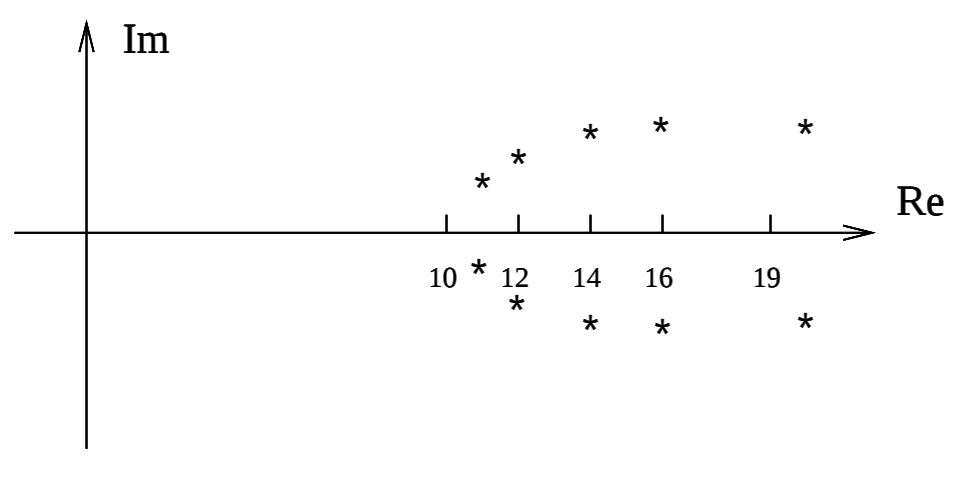
\includegraphics[width=\linewidth]{img/2/2_4_wilkinson_plot}
          \[
              \frac{
                  \partial x
              }{
                  \partial \alpha
              } = \frac{
                  \frac{\partial p}{\partial \alpha}
              }{
                  \frac{\partial p}{\partial x}
              } = \frac{
                  x^{19}
              }{
                  \sum_{i=1}^{20} \prod_{j=1, j \neq i}^{20} (x-j)
              }
          \]
          \[ 
              \left.
                  \frac{\partial x}{\partial \alpha}
              \right|_{x=1} = \frac{
                  i^{19}
              }{
                  \prod_{j=1, j \neq i}^{20}
              }, i = 1, 2, ..., 20
          \]
    	\end{column}
        \begin{column}{.3\linewidth}
          \begin{tabular}{r | l}
              i & $\left.
                  \frac{\partial x}{\partial \alpha}
              \right|_i$ \\
              \hline
               1 & $-8.2 \cdot 10^{-18}$ \\
               2 & $ 8.2 \cdot 10^{-11}$ \\
               5 & $-6.1 \cdot 10^{-1}$  \\
               6 & $ 5.8 \cdot 10^{1}$   \\
               8 & $ 6.0 \cdot 10^{4}$   \\
              10 & $ 7.6 \cdot 10^{6}$   \\
              15 & $-2.1 \cdot 10^{9}$   \\
              19 & $-3.1 \cdot 10^{8}$   \\
              20 & $ 4.3 \cdot 10^{7}$   \\
          \end{tabular}
        \end{column}
    \end{columns}
    \end{exampleblock}
\end{frame}
%%%%%%%%%%%%%%%%
	%%%%%%%%%%%%%%%%
	\section{Algorytmy numerycznie poprawne}
%%%%%%%%%%%%%%%%
\begin{frame}{Algorytmy numerycznie poprawne}
	Ograniczenia:
    \begin{itemize}
    	\item dane - {\it zaburzone}
    	\item wyniki - {\it zaburzone}
    \end{itemize}
    stąd: błędy reprezentacji
\end{frame}
%%%%%%%%%%%%%%%%
\begin{frame}{Algorytmy numerycznie poprawne}
	\begin{block}{Definicja}
		{\bf Algorytmy numerycznie poprawne} - takie, które dają rozwiązania będące nieco zaburzonym dokładnym rozwiązaniem zadania o nieco {\it zaburzonych} danych. Są to algorytmy najwyższej jakości.
        
        {\bf Dane nieco zaburzone} - zaburzone na poziomie reprezentacji.
	\end{block}
\end{frame}
%%%%%%%%%%%%%%%%
\begin{frame}{Algorytmy numerycznie poprawne - definicje}
	\begin{block}{Definicja}
    	Algorytm A jest {\bf numerycznie poprawny} w klasie zadań $K_d$, $K_w$, jeżeli istnieją stałe $K_d, K_w$ takie, że:
        \begin{itemize}
        	\item $\forall d \in D$,
            \item dla każdej dostatecznie silnej arytmetyki $\left( \beta^{1-t} \right)$
        \end{itemize}
        $\exists \tilde{d} \in D_0$ taki, że:
        
        {\centering
        	$|| \vec{d} - \tilde{d} || \le \varrho_d \cdot K_d \cdot || \vec{d} ||$ \\ \vspace{.1cm}
            $|| \varphi(\vec{d}) - fl(A(\vec{d})) || \le \varrho_w \cdot K_w \cdot || \varphi(\vec{d}) ||$ \\}

        $\varphi(\vec{d})$ - dokładnie rozwiązanie zadania o zaburzonych danych $\tilde{d}$ \\
        $K_w, K_d$ - wskaźniki kumulacji algorytmu A w klasie zadań $\left\{\varphi, D\right\}$
        $K_w, K_d$:
        \begin{itemize}
        	\item dla dowolnych danych klasy $\left\{ \varphi, D \right\}$,
            \item minimalne $\rightarrow$ jakość A.
        \end{itemize}
	\end{block}
\end{frame}
%%%%%%%%%%%%%%%%
\begin{frame}{Algorytmy numerycznie poprawne - definicje}
	\begin{block}{Definicja}
		{\bf Użyteczne algorytmy} - gdy wskaźniki kumulacji rzędu liczby działań
	\end{block}
\end{frame}
%%%%%%%%%%%%%%%%
\begin{frame}[fragile]{Algorytmy numerycznie poprawne - przykład}
	\begin{exampleblock}{Przykład 1}
		Numeryczna poprawność algorytmu $\vec{a} \cdot \vec{b} = \sum_{i=1}^{n} a_i \cdot b_i$
        
\begin{lstlisting}[escapechar=|]
  |$A(\vec{a}, \vec{b}):$|
  s := 0;
  for i:=1 to n do s := s + |$a_1 \cdot b_i$|;
\end{lstlisting}
	\end{exampleblock}
\end{frame}
%%%%%%%%%%%%%%%%
\begin{frame}{Algorytmy numerycznie poprawne - przykład}
	\begin{exampleblock}{Przykład 1}
		{\bf Realizacja algorytmu}: $fl(A(\vec{a}, \vec{b}))$:
        \begin{enumerate}
        	\item dane - reprezentacje \\
                \hspace{1cm} $a_i \to \hat{a_i} = rd(a_i) = a_i \cdot (1 + \alpha_i)$ \\
                \hspace{1cm} $b_i \to \hat{b_i} = rd(b_i) = b_i \cdot (1 + \beta_i)$
        	\item działania - przybliżone, $fl$ \\
            	np. $i = 1, 2, 3:$ \\ 
                \begin{addmargin}[1em]{0em}
                $
                    fl(A(\vec{a}, \vec{b})) = \{
                        [
                            \hat{a_1} \cdot \hat{b_1} \cdot (1 + \varepsilon_1) +
                            \hat{a_2} \cdot \hat{b_2} \cdot (1 + \varepsilon_2) +
                        ]
                        \cdot (1 + \delta_2) + \hat{a_3} \cdot \hat{b_3} \cdot (1 + \varepsilon_3)
                    \} \cdot (1 + \delta_3); 
                $ \\
                $\delta_1 = 0$ \\
                
                \end{addmargin}
            	i ogólnie:
                \begin{addmargin}[1em]{0em}
                $
                	fl(A(\vec{a}, \vec{b})) =
                	\sum_{i=1}^{n} a_i \cdot (1+a_i) \cdot 
                    b_i \cdot (1 + \beta_i) \cdot (1 + \varepsilon_i)
                    \cdot \prod_{j=i}^{n} (1 + \delta_j)
                $                
                \end{addmargin}
        \end{enumerate}
	\end{exampleblock}
\end{frame}
%%%%%%%%%%%%%%%%
\begin{frame}[fragile]{Algorytmy numerycznie poprawne - przykład}
	\begin{exampleblock}{Przykład 1}
    	{\bf Interpretacja (dowolność)}
        \begin{itemize}
        	\item dokładny wynik: $K_w = 0$
            \item dla zaburzonych danych:
            	\begin{addmargin}[1cm]{0cm}
            		$|| \vec{a} - \tilde{a} || \le \beta^{1-t} \cdot || \vec{a} ||$ \hspace{.5cm} $(K_{d_1} = 1)$\\
            		$|| \vec{b} - \tilde{b} || \le (n + 1) \cdot \beta^{1-t} \cdot || \vec{b} ||$ \hspace{.5cm} $(K_{d_2} = n+1)$
            	\end{addmargin}
        \end{itemize}
        {\bf Uwaga:} pominięcie błędów reprezentacji danych $\equiv$ zmniejszenie $K_d$ o 1.
	\end{exampleblock}
\end{frame}
%%%%%%%%%%%%%%%%
	%%%%%%%%%%%%%%%%
	\section{Stabilność numeryczna}
%%%%%%%%%%%%%%%%
\subsection{Przykłady}
%%%%%%%%%%%%%%%%
\begin{frame}{Stabilność numeryczna - przykłady}
	\begin{exampleblock}{Przykład 1}
    \setstretch{.5}
    \fontsize{9}{9}
      \begin{columns}[T]
      	\column{.25\linewidth}
        \vspace{.5cm}
            \[
                e^x = 1 + x + \frac{x^2}{2!} + \frac{x^3}{3!} + ...
            \]\[
                \beta = 10, t = 5, x = -5.5
            \]\newline
            \[
            	e^{x}=\sum_{n=0}^{\infty}\frac{x^{n}}{n!}
            \]
		\column{.65\linewidth}
          \begin{columns}
              \column{.55\linewidth}
                  \begin{align*}
                      e^{-5.5}  	=& &   1&.0 \\
                                   & &  -5&.5 \\
                                   & & +15&.125 \\
                                   & & -27&.730 \\
                                   & & +38&.129 \\
                                   & & -41&.942 \\
                                   & & +38&.446 \\
                                   & & -30&.208 \\
                                   & & +20&.768 \\
                                   & & -12&.692 \\
                                   & &  +6&.9803 \\
                                   & &  -3&.4902 \\
                                   & &  +1&.5997 \\
                                   & & .&..\\
                                   \hline \\[-8pt]
                                   & &   0&.0026363
                  \\[-7pt]
                  \text{\bf ALE  } e^{-5.5} =& & 0&.00408677 \hspace{3pt} !
                  \end{align*}
              \column{.38\linewidth}
                  25 składników \\i brak zmian \\w sumie
          \end{columns}
      \end{columns}
	\end{exampleblock}
\end{frame}
%%%%%%%%%%%%%%%%
\begin{frame}{Stabilność numeryczna - przykłady}

	\begin{exampleblock}{Przykład 1}
        {\bf Przyczyna:} np. 38.129 $\Rightarrow$ błąd reprezentacji $\approx$ wynik! ({\it catastrophic cancellation})\\
        Sposób obliczeń wzmacniający błędy reprezentacji!\\
        A co dla $e^{-200}$?\\
        Po zmianie algorytmu: ($\beta, t$ - j.w.)
        \\[-6pt]
        \[
            e^{-5.5} = \frac{1}{e^{5.5}} = \frac{1}{1 + 5.5 + 15.125 + ...} = \underbrace{0.0040865}_\text{0.007\%!}
        \]
        \\[-8pt]
        $e^x$ oblicza się:
        \\[-18pt]
        \begin{align*}
                         x &= m + f, \text{m - całkowite, } 0 \le f < 1 \\
                         e^x &= e^{m+f} = e^m \cdot e^f \\
            \text{lub }  e^x &= e^{(1 + \frac{f}{m}) \cdot m} = \left[ e^{1 + \frac{f}{m}} \right]^m
        \end{align*}
    \end{exampleblock}
\end{frame}
%%%%%%%%%%%%%%%%
\begin{frame}{Stabilność numeryczna - przykłady}
	\begin{exampleblock}{Przykład 2}
    \setstretch{.7}
		\[
        	E_n = \int_0^1 x^n \cdot e^{x-1} dx, \hspace{.5cm} n = 1, 2, ...
        \]
        całkowanie przez części:
        \\[-15pt]
		\begin{align*}
			& \int_0^1 x^n \cdot e^{x-1} dx = 
            \left. x^n \cdot e^{x-1}
            \right|_0^1 - \int_0^1 n \cdot x^{n-1} \cdot e^{x-1} dx \\
            & \Rightarrow
            \left\{
            	\begin{array}{ll}
            		E_n = 1-n \cdot E_{n-1}, \hspace{.5cm} n = 2, 3, ... \\
                    E_1 = \frac{1}{e}
            	\end{array}
            \right.
		\end{align*}
        \\[-5pt]
        $\beta = 10, t = 6$
        \\[-13pt]
        \begin{align*}
        	E_1 &\approx 0.367879, \varepsilon \approx 4.412 \cdot 10^{-7} \\
            E_2 &\approx 0.264242 \\
            ... \\
            E_8 &\approx 0.118720 \\
            E_9 &\approx -0.0684800 \hspace{.3cm} !! \hspace{.3cm} \text{Bo: } x^9 \cdot e^{x-1} \ge 0, x \in [0, 1]
        \end{align*}
	\end{exampleblock}
\end{frame}
%%%%%%%%%%%%%%%%
\begin{frame}{Stabilność numeryczna - przykłady}
	\begin{exampleblock}{Przykład 2}
		Powód $\rightarrow \varepsilon(E_1):$
        \begin{align*}
        	\text{w } E_2 &\rightarrow \varepsilon \cdot 2 \\
        	\text{w } E_3 &\rightarrow \varepsilon \cdot 2 \cdot 3 \\
            ... \\
            \text{w } E_9 &\rightarrow \varepsilon \cdot 2 \cdot 3 \cdot 4 \cdot ... \cdot 9 = \varepsilon \cdot 9! = \varepsilon \cdot 362880 \approx 0.1601
        \end{align*}
        i nawet: $-0.06848 + 0.1601 = 0.0916$ - poprawny!
	\end{exampleblock}
\end{frame}
%%%%%%%%%%%%%%%%
\begin{frame}{Stabilność numeryczna - przykłady}
	\begin{exampleblock}{Przykład 2}
    Jak wybrać dobry (stabilny) algorytm?
    \\[-10pt]
    \[
    	E_{n-1} = \frac{1 - E_n}{n}, \hspace{.3cm} n = ..., 3, 2.
    \]
    \\[-8pt]
    Na każdym etapie zmniejszamy błąd $n$ razy - {\bf algorytm stabilny}.
    \\[-20pt]
    \begin{align*}
    	E_n = \int_0^1 x^n \cdot e^{x-1} dx \le \int_0^1 x^n dx =
        \left.
        	\frac{x^{n+1}}{n+1}
        \right|_0^1 = \frac{1}{n+1} \\
        \lim_{n \to \infty} E_n = 0 \\
        E_{20} \approx 0.0 \hspace{.3cm} \text{- błąd } \hspace{.1cm} \frac{1}{20} \\
        E_{19} \rightarrow \frac{1}{20} \cdot \frac{1}{21} \approx 0.0024 \\
        \\[-22pt]
        ... \\
        E_{15} \approx 0.0590176 \rightarrow \text{wartość dokładna na 6 miejscach znaczących.}
    \end{align*}
    \end{exampleblock}
\end{frame}
%%%%%%%%%%%%%%%%
\begin{frame}{Stabilność numeryczna - przykłady}
	\begin{block}{Przykład 2 - definicja}
		Metoda numerycznie jest {\bf stabilna}, jeżeli mały błąd na dowolnym etapie przenosi się dalej z {\it malejącą amplitudą}.
        \[
        	\varepsilon^{n+1} = g \cdot \varepsilon^n \hspace{.2cm} 
            \Rightarrow \text{stabilna:}
            \left| \varepsilon^{n+1} \right| \le \left| \varepsilon^n \right|, \hspace{.2cm} g \text{ - wsp. wzmocnienia}
        \]
	\end{block}
	\textbf{Uwaga:} $\newline$
	Jakość wyniku poprawia się wraz z każdym kolejnym etapem obliczeń.
\end{frame}
%%%%%%%%%%%%%%%%
\subsection{Definicja}
%%%%%%%%%%%%%%%%
\begin{frame}{Stabilność numeryczna - definicja}
	\begin{block}{Definicja}
    	{\bf Algorytm najwyższej jakości} - algorytm numerycznie poprawny.
    \end{block}
    \vspace{-20pt}
    \begin{align*}
    	\vec{w} = \varphi(\vec{d}) &\\
        \hat{d}: ||\vec{d} - \hat{d}|| \le \varrho_d ||\vec{d} || &,&& 
        	\hat{d} - \text{dane zaburzone na poz. repr.} \\
        \hat{w} = \varphi(\hat{d}) &,&&
        	\hat{w} - \text{dokł. rozw. dla danych zab.} \\
		\tilde{w}: ||\hat{w} - \tilde{w} || \le \varrho_w ||\tilde{w}|| &,&&
        	\tilde{w} - \text{wynik dla $\hat{d}$,} \\
            &&&\text{zab. na poz. reprezentacji} \\
        ||\vec{w} - \tilde{w} || \le ||\vec{w} - \hat{w}|| + ||\hat{w} - \tilde{w}|| &\le&&
        	(1 + \varrho_w) \cdot \max_{\hat{d}} ||\varphi(\vec{d}) - \varphi(\hat{d})|| +\\
            &&&+ \varrho_w ||\vec{w}|| \\
        P(\vec{d}, \varphi) &=&& \varrho_w ||\vec{w}|| + \max_{\hat{d}} ||\varphi(d) - \varphi(\hat{d})||
    \end{align*}
\end{frame}
%%%%%%%%%%%%%%%%
\begin{frame}{Optymalny poziom błędu rozwiązania $\varphi(\vec{d})$ w arytmetyce $fl$}
	\begin{block}{Definicja}
		Algorytm A nazywamy {\bf numerycznie stabilnym} w klasie $\{\varphi, D\}$, jeżeli istnieje stała $K$ taka, że 
        \begin{itemize}
        	\item $\forall \vec{d} \in D$,
            \item dla każdej dostatecznie silnej arytmetyki
        \end{itemize}
        zachodzi:
        \[
        	||\varphi(\vec{d}) - fl(A(\vec{d}))|| \le \underbrace{K}_\text{małe} \cdot P(\vec{d}, \varphi)
        \]
        {\bf numerycznie poprawny} - stabilny (minimalny wymóg)
	\end{block}
\end{frame}
	%%%%%%%%%%%%%%%%
	\section{Złożoność obliczeniowa {\it computational complexity}}
%%%%%%%%%%%%%%%%
\begin{frame}{Złożoność obliczeniowa}
	Oprócz jakości algorytmu - ważny jego {\it koszt} - liczba działań arytmetycznych (logicznych) potrzebnych do rozwiązania zadania - algorytmy minimalizujące liczbę działań.
\end{frame}
%%%%%%%%%%%%%%%%
\begin{frame}{Rezultaty}
	\begin{enumerate}
		\item Oszacowanie złożoności obliczeniowej ,,z dołu'': jeżeli zadanie ma $n$ danych istotnych, to minimalna liczba działań arytmetycznych potrzebnych do obliczenia wyniku:
        \[
        	z(\varphi, D) \ge \frac{n}{2}
        \]
        \item Dla wielu zadań można udowodnić, że minimalna liczba działań w algorytmie numerycznie poprawnym musi być istotnie większa od liczby danych.
        \item Metody optymalne co do $z(\varphi, D)$ znane są dla niewielu, prostych zadań.
	\end{enumerate}
\end{frame}
%%%%%%%%%%%%%%%%
\begin{frame}{Złożoność obliczeniowa - przykład}
	\begin{exampleblock}{Przykład}
        \begin{itemize}
            \item prosty
            \item ilustruje konieczność myślenia {\it do końca} przy wyborze algorytmu
        \end{itemize}
        {\bf Zadanie:}
        \[
        	S = \sum_{i=1}^n (-1)^i \cdot i;
        \]
	\end{exampleblock}
\end{frame}
%%%%%%%%%%%%%%%%
\begin{frame}[fragile]{Złożoność obliczeniowa - przykład}
	\begin{exampleblock}{Przykład}
    	{\bf A1:}
    	\begin{lstlisting}[escapechar=|]
s = 0
do 1 i=1, n
    s = s+(-1)**i*i
continue \end{lstlisting}
		\vspace{-15pt}
    	{\bf A2:}
    	\begin{lstlisting}[escapechar=|]
s = 0
do 1 i=1,n,2
    s = s-1
continue
do 1 i=1,n,2
	s = s+1
continue \end{lstlisting}
		\vspace{-15pt}
	\end{exampleblock}
\end{frame}
%%%%%%%%%%%%%%%%
\begin{frame}[fragile]{Złożoność obliczeniowa - przykład}
	\begin{exampleblock}{Przykład}
    	{\bf A3:}
    	\begin{lstlisting}[escapechar=|]
s = n/2
if (mod(n,2).eq.1) s=-s \end{lstlisting}
		\vspace{-15pt}
        \begin{itemize}
        	\item ilość operacji nie zależy od $n$
            \item nie ma akumulacji błędów
            \item nie grozi overflow
        \end{itemize}
	\end{exampleblock}
\end{frame}
	%%%%%%%%%%%%%%%%
	\section{Zadania}
%%%%%%%%%%%%%%%%
\begin{frame}{Zadania}
	Elementy analizy:
    \begin{itemize}
    	\item Tw. Rolle'a
        \item Tw. o wartości średniej
        \item Tw. o wartości średniej dla całek
        \item Tw. Taylor'a
    \end{itemize}
\end{frame}
%%%%%%%%%%%%%%%%
\begin{frame}{Zadania}
	Zbadać uwarunkowanie zadania (wskaźniki uwarunkowania):
    \begin{enumerate}
    	\item wyznaczania zer wielomianu: \[
				P(x) = \sum_{i/0}^{20} a_i x^i = \prod_{i/0}^{20} (x-i)
            \]
        \item wyznaczenia zer rzeczywistych: \[
        		x^2 - 2px + q = 0, \hspace{.2cm} p, q \in D = \{ 
                	(p, q): p \neq 0, q \neq 0, p^2 - q > 0
                \}
        	\]
    \end{enumerate}
\end{frame}
%%%%%%%%%%%%%%%%
\begin{frame}{Zadania}
	Sprawdzić poprawność numeryczną:
    \begin{enumerate}
    	\item algorytmu Herona $x = \sqrt{a}$
        	\begin{align*}
                x_1 &= \left\{
                    \begin{array}{ll}
                        a, \hspace{.3cm} a \ge 1 \\
                        1, \hspace{.3cm} a < 1
                    \end{array}
                \right. \\ 
                x_{i+1} &= \frac{1}{2}(x_i + \frac{a}{x_i}), i=1, 2, ...
        	\end{align*}
        \item algorytmu Hornera \[
        	P(x) = (...(a_n x + a_{n-1} x)x + ... + a_1) x + a_0
        \]
    \end{enumerate}
\end{frame}
	%%%%%%%%%%%%%%%%

\end{document}
